%================================================================%
%=============  Modelo de Trabalho de Conclusão de curso ========%
%========================  IFMG =================================% 
% AUTORES:
% prof. Elias J R Freitas =======================================%
% ej-ensino.com.br
%
% baseado no modelo DEPRO-UFOP 
% estrutura elaborada inicialmente por
% Marcelus Xavier Oliveira  e Dayanne Gouveia Coelho ===============%

%================================================================%
% Proposta de texto em conformidade com normas da ABNT ----------%
% Modelo em conformidade com 
% Manual de Normalização de Trabalhos Acadêmicos 21/02/2020
% https://www.ifmg.edu.br/portal/ensino/bibliotecas/
% arquivos-bibliotecas/copy_of_ManualdeNormalizaoIFMG2020.pdf
% implementadas pelo projeto abntex2, que pode ser acessado pela %
% página  http://abntex2.googlecode.com/  -----------------------%
%================================================================%

%================================================================%
% Versao abntex2
%======================== Versão 2022/02 ========================%
%================================================================%


\documentclass[12pt, % tamanho da fonte
	%openright,	% capítulos começam em pág ímpar
	oneside, %para impressão apenas em um lado (formato digital).  		  
	% twoside, %para impressão em frente e verso.  
	a4paper,			% tamanho do papel. 
	english,			% Idioma adicional para hifenização
	brazil				% Idioma principal 
	]{packages/abntex2-ifmg}
	
%------------------------------------------------------------
%------------    Estrutura do texto   -----------------------         

% Pacotes Básicos:
%\usepackage{lmodern}			    % Usa a fonte Latin Modern			
\usepackage{pslatex}                % Usa a fonte Times New Roman
\usepackage[T1]{fontenc}		  % Selecao de codigos de fonte.
\usepackage[utf8]{inputenc}		% Codificacao do documento (conversão automática dos acentos)
\usepackage{lastpage}			    % Usado pela Ficha catalográfica
\usepackage{indentfirst}		  % Indenta o primeiro parágrafo de cada seção.
\usepackage[table]{xcolor}
\usepackage{color}				    % Controle das cores
\usepackage{graphicx}			    % Inclusão de gráficos
\usepackage{microtype} 		  	% para melhorias de justificação

\usepackage{tablefootnote} % para colocar footnotes em tabelas e figuras

% Pacotes Extras:
\usepackage[final]{pdfpages}
\usepackage{amsmath,amsthm}   %Símbolos Matemáticos
\usepackage{indentfirst} % Indenta primeiro parágrafo 
\usepackage[portuguese, ruled, linesnumbered,commentsnumbered, algo2e, vlined, lined, boxed, algochapter]{algorithm2e} % Algoritmos 
\usepackage{hyperref}
\usepackage[brazilian,hyperpageref]{backref}	 % Paginas com as citações na bibliograficas


%\usepackage[num]{abntex2cite}	% Citações padrão ABNT númerico
\usepackage[alf,abnt-emphasize=bf,abnt-full-initials=no,abnt-etal-list=5,abnt-etal-text=emph,abnt-repeated-author-omit=yes]{abntex2cite}
%\usepackage[alf,abnt-emphasize=bf,abnt-etal-list=0,abnt-etal-text=emph]{abntex2cite}

% se desejar justificar as referências (pela abnt é alinhado a esquerda)
% \usepackage[alf,abnt-emphasize=bf,bibjustif]{abntex2cite}

\usepackage{float} % para ajustar a posição das imagens

\usepackage{tikzsymbols} %para caracteres emoji
\usepackage{stackengine}
\usepackage{scalerel}

\newcommand\dangersign[1][2ex]{%
  \renewcommand\stacktype{L}%
  \scaleto{\stackon[1.3pt]{\color{red}$\triangle$}{\tiny\bfseries !}}{#1}%
}

\usepackage{etoolbox}
%\usepackage[num]{abntex2cite}  % Citações numéricas

\usepackage{lipsum}

%para usar os algoritmos e matematica
\newcommand{\var}{\texttt}

\usepackage{amssymb}
\usepackage{amsmath}



% Defininfo Cores:
\definecolor{blue}{RGB}{25,25,112}
\definecolor{midgray}{gray}{.7}

\makeatletter % informações do PDF
\hypersetup{ % pagebackref=true,
	pdftitle={\@title}, 
	pdfauthor={\@author},
    pdfsubject={\imprimirpreambulo},
	pdfcreator={LaTeX with abnTeX2},
	pdfkeywords={abnt}{latex}{abntex}{abntex2}{trabalho acadêmico}, 
	colorlinks=true,     % false: boxed links; true: colored links
    linkcolor=black,          	% color of internal links
    citecolor=black,        		% color of links to bibliography
    filecolor=magenta,      	% color of file links
    urlcolor=black,
	bookmarksdepth=4 }
\makeatother
 

% -------------------------------------------- 
% Espaçamentos entre linhas e parágrafos 
\setlength{\parindent}{1.3cm} % O tamanho do parágrafo

% Controle do espaçamento entre um parágrafo e outro:
\setlength{\parskip}{0.2cm}  % tente também \onelineskip

% Definição de ambientes matemáticos em português 
\newtheorem{teorema}{Teorema}[chapter]
\newtheorem{axioma}{Axioma}[chapter]
\newtheorem{corolario}{Corolário}[chapter]
\newtheorem{lema}{Lema}[chapter]
\newtheorem{proposicao}{Proposição}[chapter]
\newtheorem{definicao}{Definição}[chapter]
\newtheorem{exemplo}{Exemplo}[chapter]
\newtheorem{observacao}{Observação}[chapter]

% Novos Comandos
\usepackage{tgtermes}
\renewcommand{\ABNTEXchapterfont}{\rmfamily\bfseries}

% Variáveis adicionais
\providecommand{\imprimirautorcite}{}
\newcommand{\autorcite}[1]{\renewcommand{\imprimirautorcite}{#1}} 
\providecommand{\imprimirsigla}{}
\newcommand{\sigla}[1]{\renewcommand{\imprimirsigla}{#1}}
\providecommand{\imprimiruf}{}
\newcommand{\uf}[1]{\renewcommand{\imprimiruf}{#1}}
\providecommand{\imprimircurso}{}
\newcommand{\curso}[1]{\renewcommand{\imprimircurso}{#1}}
\providecommand{\imprimirinstituto}{}
\newcommand{\instituto}[1]{\renewcommand{\imprimirinstituto}{#1}}
\providecommand{\imprimirdepartamento}{}
\newcommand{\departamento}[1]{\renewcommand{\imprimirdepartamento}{#1}}
\providecommand{\imprimirano}{}
\newcommand{\ano}[1]{\renewcommand{\imprimirano}{#1}}
\providecommand{\imprimirdia}{}
\newcommand{\dia}[1]{\renewcommand{\imprimirdia}{#1}}
\providecommand{\imprimirmes}{}
\newcommand{\mes}[1]{\renewcommand{\imprimirmes}{#1}}
\providecommand{\imprimirgrau}{}
\newcommand{\grau}[1]{\renewcommand{\imprimirgrau}{#1}}
\providecommand{\imprimirexaminadorum}{}
\newcommand{\examinadorum}[1]{
    \renewcommand{\imprimirexaminadorum}{#1}}
\providecommand{\imprimirexaminadordois}{}
\newcommand{\examinadordois}[1]{
    \renewcommand{\imprimirexaminadordois}{#1}}
\providecommand{\imprimirexaminadortres}{}
\newcommand{\examinadortres}[1]{
    \renewcommand{\imprimirexaminadortres}{#1}}
\providecommand{\imprimirexaminadorquatro}{}
\newcommand{\examinadorquatro}[1]{
    \renewcommand{\imprimirexaminadorquatro}{#1}}
\providecommand{\imprimirttorientador}{}
\newcommand{\ttorientador}[1]{
    \renewcommand{\imprimirttorientador}{#1}} 
\providecommand{\imprimirttcoorientador}{}
\newcommand{\ttcoorientador}[1]{
    \renewcommand{\imprimirttcoorientador}{#1}}
\providecommand{\imprimirttexaminadorum}{}
\newcommand{\ttexaminadorum}[1]{
    \renewcommand{\imprimirttexaminadorum}{#1}}
\providecommand{\imprimirttexaminadordois}{}
\newcommand{\ttexaminadordois}[1]{\renewcommand{
        \imprimirttexaminadordois}{#1}}
\providecommand{\imprimirttexaminadortres}{}
\newcommand{\ttexaminadortres}[1]{
    \renewcommand{\imprimirttexaminadortres}{#1}}
\providecommand{\imprimirttexaminadorquatro}{}
\newcommand{\ttexaminadorquatro}[1]{
    \renewcommand{\imprimirttexaminadorquatro}{#1}}

% Cria o comando \subtitulo. A norma define que o TITULO deve ser em caixa alta
% negrito, mas o subtitulo deve ser em caixa baixa.
\providecommand{\imprimirsubtitulo}{}
\newcommand{\subtitulo}[1]{\renewcommand{\imprimirsubtitulo}{#1}}

%----------------------------------------------------
\renewcommand{\imprimircapa}{  % Capa 
\begin{capa}
%\begin{center}
\includegraphics[scale=1]{Figuras/ifmg.png}\end{center}
\begin{center}{
             \large \MakeTextUppercase{\imprimirinstituicao} - \MakeTextUppercase{\imprimirinstituto} \\
              %\imprimirdepartamento \\
              \MakeTextUppercase{\imprimircurso} \\
              \vspace{2cm}
			  \large {\imprimirautor} 
			  }\end{center}
\vfill
        \begin{center}
        \MakeTextUppercase{\large \textbf{\imprimirtitulo}}  \\
        \MakeTextLowercase{\textbf{\imprimirsubtitulo}}
				\vspace{2cm}
				%{\large \imprimirautor} 	
				\vfill
        {\large{\imprimirlocal~-~\imprimiruf \\ \imprimirano }}
        \end{center}
\end{capa}   } % Capa

%----------------------------------------------------
\renewcommand{\imprimirfolhaderosto}{% folha de rosto
    \begin{center}
    {{\MakeTextUppercase \imprimirautor}}  \\
		\vfill
		\large {\textbf{\MakeTextUppercase{\imprimirtitulo}}\\
        \MakeTextLowercase{\textbf{\imprimirsubtitulo}}}
    \end{center}
    \vfill 
    \begin{flushright} 
    \parbox{0.6\linewidth}{
		\imprimirtipotrabalho~ apresentado ao Curso de \imprimircurso~ do \imprimirinstituicao~ - \imprimirinstituto~ para a obtenção do título de \imprimirgrau. \\
		\vfill
		\textbf{\imprimirorientadorRotulo}~\imprimirorientador \\
		\vfill 
		\textbf{\imprimircoorientadorRotulo}~\imprimircoorientador}
   \end{flushright} 
   
	 \vfill
   \begin{center}
   {\large{\imprimirlocal~- \imprimiruf \\ \imprimirano}}
   \end{center} }  % folha de rosto

%----------------------------------------------------


%================================================================================
% Pacotes de citações
%================================================================================

% Configurações do pacote backref
% Texto padrão antes do número das páginas
\renewcommand{\backref}{}
% Define os textos da citação
\addto\captionsbrazil{% portugues-brasil
    % Usado sem a opção hyperpageref de backref
    \renewcommand{\backrefpagesname}{Citado na(s) p{\'a}gina(s):~}
    \renewcommand*{\backrefalt}[4]{
    	\ifcase #1 %
    		Nenhuma cita{\c c}{\~a}o no texto.%
    	\or
    		Citado na p{\'a}gina #2.%
    	\else
    		Citado #1 vezes nas p{\'a}ginas #2.%
    	\fi}%
}
\addto\captionsenglish{% ingles
    % Usado sem a opção hyperpageref de backref
    \renewcommand{\backrefpagesname}{Cited on page(s):~}
    \renewcommand*{\backrefalt}[4]{
    	\ifcase #1 %
    		No citation.%
    	\or
    		Cited on page #2.%
    	\else
    		Cited #1 times on pages #2.%
    	\fi}%
}
% ---
\makeatletter
\newcommand\thefontsize{Fonte tamanho: \f@size pt}
\makeatother



% para não deixar uma figura sozinha no centro de uma página,
% mas no topo da página.
\makeatletter
\setlength{\@fptop}{0pt}
\makeatother




%--  % Estrutura do Texto e Pacotes Principais

% -- Informações para Capa e Folha de Rosto a serem editadas

\titulo{Título do trabalho:} 
% caso o trabalho não tenha subtítulo comentar linha abaixo e retirar dois pontos do título do trabalho
\subtitulo{Subtítulo do trabalho}

\autor{Nome Completo do Aluno} \autorcite{SOBRENOME, Nome}
\local{Ibirité} \uf{MG}
\data{21 de Fevereiro de 2022} \dia{21} \mes{02} \ano{2022} %deixar sem preencher antes do TCC
\orientador{Prof. Dr. Nome do orientador}  % Nome do orientador 
\ttorientador{IFMG} % Instituição do orientador
\coorientador{Prof. Me. Nome do Coorientador}   % Nome do coorientador
\ttcoorientador{IFMG} % Instituição do Coorientador
\instituicao{Instituto Federal de Educação, Ciência e Tecnologia de Minas Gerais} \sigla{IFMG}
\instituto{\textit{Campus} Ibirité}
%\departamento{Departamento de Engenharia de Controle e Automação e Técnicas Fundamentais}
\curso{Engenharia de Controle e Automação}	
\tipotrabalho{Trabalho de conclusão de curso}
\grau{Engenheiro de Controle e Automação}

%------Nomes dos examinadores.  
\examinadorum{Prof. Me. Membro da Banca 1} \ttexaminadorum{UFXX}
\examinadordois{Prof. Dr. Membro da Banca  2} \ttexaminadordois{IFMG}
%\examinadortres{Prof. Dr. Membro da Banca  3} \ttexaminadortres{Universidade Federal de ... - UFXX}
%\examinadorquatro{Prof. Dr. Membro da Banca  4} \ttexaminadorquatro{Universidade Federal de ... - UFXX}

% ------------------------------------------------------
\makeindex   

\begin{document} % Início do documento

\frenchspacing  % Retira espaço obsoleto entre as frases.

% ----------------------------------------------------------
% -- Elementos Pré-Textuais: -------------------------------
\pagenumbering{roman}

\imprimircapa  % Capa
\imprimirfolhaderosto % Folha de rosto

% ---------------------------------------------------------------
% ----------------  Ficha Catalográfica  -------------------------
% ---------------------------------------------------------------
% Modelo de ficha catalográfica. Você deverá substituir esta
% folha na versão final da monografia por um pdf fornecido pela 
% biblioteca. Salve o modelo oficial como ficha_catalografica.pdf
% e use o comando abaixo para inseri-lo na versão final do texto.

%\begin{fichacatalografica}
%    \includepdf{ficha_catalografica.pdf}
%\end{fichacatalografica}



%% Modelo de Como fazer a Ficha Catalográfica:

\begin{fichacatalografica}
	\sffamily
	\vspace*{\fill}					% Posição vertical
	\begin{center}					% Minipage Centralizado
	\fbox{\begin{minipage}[c][8cm]{13.5cm}		% Largura
	
	Ficha catalográfica a ser fornecida pela biblioteca.
% 	\small
% 	\imprimirautorcite.
% 	%Sobrenome, Nome do autor
	
% 	\hspace{0.5cm}  \\
% 	\imprimirtitulo  / \imprimirautor. --, \imprimirano-
	
% 	\hspace{0.5cm} \pageref{LastPage} p. 1 :il. (colors; grafs; tabs).\\
	
% 	\hspace{0.5cm} \imprimirorientadorRotulo~\imprimirorientador\\
	
% 	\hspace{0.5cm}
% 	\parbox[t]{\textwidth}{\imprimirtipotrabalho~--\\ \imprimirinstituicao. \\
% 	\imprimirinstituto. \\ ~\imprimirdepartamento.}\\
	
% 	\hspace{0.5cm}
% 		1. Palavra-chave1.
% 		2. Palavra-chave2.
% 		2. Palavra-chave3.
% 		I. \imprimirorientador.
% 		II. \imprimirinstituicao.
% 		III. Título 			
	\end{minipage}}
	\end{center}
\end{fichacatalografica}



% ---------------------------------------------------------------
% ----------------  Folha de aprovação  -------------------------
% ---------------------------------------------------------------
% Modelo de Folha de aprovação. Você deverá substituir esta
% folha na versão final da monografia por um pdf fornecido pelo  
% colegiado do seu curso. Salve o modelo oficial como 
% folhadeaprovacao_final.pdf e use o comando abaixo para
% inseri-lo na versão final do texto.

%\begin{fichacatalografica}
%    \includepdf{folhadeaprovacao_final.pdf}
%\end{fichacatalografica} Esta folha será 


\begin{folhadeaprovacao}

\begin{center}
    \large { \imprimirautor}  \\
		\vspace{3cm} 
		\large {\textbf{\MakeTextUppercase{\imprimirtitulo}}~\MakeTextLowercase{\imprimirsubtitulo}}
    \end{center}
    \vspace{2cm}
    \begin{flushright} 
    \parbox{0.6\linewidth}{
		\imprimirtipotrabalho~ apresentado ao Curso de \imprimircurso~ do \imprimirinstituicao~ - \imprimirinstituto~ para a obtenção do título de \imprimirgrau. \\
		}
   \end{flushright} 
  % \vspace{2cm}
   \vfill
 
   \begin{center}
   \large{
   Aprovado em:~\imprimirdia /\ \imprimirmes/\ \imprimirano~ pela banca examinadora:
    \vspace{2cm}
    \vfill
          \rule{15cm}{.1pt} \\
      {\imprimirorientador}~-~{\imprimirttorientador}~(Orientador) 
      \vfill
			 \ifdefvoid{\imprimircoorientador}{}{
      \rule{15cm}{.1pt} \\
      \imprimircoorientador~-~\imprimirttcoorientador~(Coorientador) }
			 \vfill
      \rule{15cm}{.1pt} \\
      {\imprimirexaminadorum}~-~{\imprimirttexaminadorum} %\\ Examinador
        \vfill
        \ifdefvoid{\imprimirexaminadordois}{}{
        \rule{15cm}{.1pt} \\
        \imprimirexaminadordois~-~\imprimirttexaminadordois %\\ Examinador
        }
				\vfill
        \ifdefvoid{\imprimirexaminadortres}{}{
        \rule{15cm}{.1pt} \\
        \imprimirexaminadortres~-~\imprimirttexaminadortres %\\ Examinador
        }
				\vfill
        \ifdefvoid{\imprimirexaminadorquatro}{}{
        \rule{15cm}{.1pt} \\
        \imprimirexaminadorquatro~-~\imprimirttexaminadorquatro %\\ Examinador
        }
   
   }
   \end{center} 

% \begin{center}
%     {\large \textsc{\imprimirautor}} \\
%   	\vspace{2cm}	
%     {\textsc{\Large \textbf{\imprimirtitulo}}} \\
% 		\vspace{2cm}
% \end{center}		

% \noindent \imprimirtipotrabalho~ defendido e aprovado em \imprimirlocal,~ \imprimirdata~,  pela banca examinadora constituída pelos professores:
% \vspace{2cm}
% \begin{center}

%       \rule{10cm}{.1pt} \\
%       {\imprimirorientador} \\ {\imprimirttorientador} \\
% 			 Orientador 
%       \vfill
% 			 \ifdefvoid{\imprimircoorientador}{}{
%       \rule{10cm}{.1pt} \\
%       \imprimircoorientador \\ \imprimirttcoorientador \\ Coorientador }
% 			 \vfill
%       \rule{10cm}{.1pt} \\
%       {\imprimirexaminadorum} \\ {\imprimirttexaminadorum} \\ Examinador
%         \vfill
%         \ifdefvoid{\imprimirexaminadordois}{}{
%         \rule{10cm}{.1pt} \\
%         \imprimirexaminadordois \\ \imprimirttexaminadordois \\ Examinador}
% 				\vfill
%         \ifdefvoid{\imprimirexaminadortres}{}{
%         \rule{10cm}{.1pt} \\
%         \imprimirexaminadortres \\ \imprimirttexaminadortres \\ Examinador}
% 				\vfill
%         \ifdefvoid{\imprimirexaminadorquatro}{}{
%         \rule{10cm}{.1pt} \\
%         \imprimirexaminadorquatro \\ \imprimirttexaminadorquatro \\ Examinador}
% \end{center}
  
\end{folhadeaprovacao}
% --- 

\begin{dedicatoria}
   \vspace*{\fill}
   \begin{flushright} 
        \parbox{0.6\linewidth}{
		 {
		Dedico esta monografia aos meus amados pais, maiores incentivadores e fontes inesgotáveis de apoio, amor e compreensão. (opcional)
		}
		}
   \end{flushright} 
   \vspace{2cm}
	 
\end{dedicatoria}
\begin{agradecimentos}

Agradeço a toda à minha família, meus pais e meu irmão agradeço por
acreditarem em mim e pelo incentivo constante na realização deste trabalho.

Agradeço ao meu orientador e a todos que contribuíram de alguma forma
para a realização deste trabalho. (opcional)

\end{agradecimentos}
\begin{epigrafe}
    \vspace*{\fill}
	\begin{flushright}
	    \parbox{0.6\linewidth}{
		“Education is not preparation for life; education is life it self." \\
		
		John Dewey
	}
	\end{flushright}
	\vspace{2cm}
\end{epigrafe}
%--------------------------------------------------------------------------
%--------------------- Resumo em Português --------------------------------
%--------------------------------------------------------------------------

%\setlength{\absparsep}{18pt} % ajusta o espaçamento dos parágrafos do resumo
\begin{resumo}
O resumo é um pequeno texto onde o autor ressalta informações importantes sobre o
trabalho, como o objetivo, resultado, métodos utilizados e conclusão ou considerações finais.
O texto do mesmo precisa ser escrito de forma clara e objetiva, preferencialmente na terceira
pessoa do singular e em voz ativa, bem como deve conter entre 150 a 500 palavras e ser redigido com espaçamento de 1,5 entre linhas.
A palavra “RESUMO” é escrita em letras maiúsculas negritadas, centralizada na margem
superior da folha.
Após o resumo devem ser incluídas as palavras-chave. Recomenda-se a utilização de no
mínimo três e no máximo cinco palavras-chave que definam o assunto do trabalho, separadas
por ponto (.).

 \vspace{\onelineskip}
 \noindent
 \textbf{Palavras-chave}: Palavra-chave1. Palavra-chave2. Palavra-chave3. 
\end{resumo}

%--------------------------------------------------------------------------
%--------------------- Resumo em Inglês --------------------------------
%--------------------------------------------------------------------------
\begin{resumo}[\large ABSTRACT]
 \begin{otherlanguage*}{english}
   É a versão em língua estrangeira do resumo em língua portuguesa, com as mesmas características, para o idioma de divulgação internacional. O resumo em língua estrangeira deve ser apresentado em folha separada, seguido das palavras-chave, separadas por ponto (.). 
   O título deve ser escrito em letras maiúsculas negritadas, centralizada na margem superior da folha.
   No IFMG, optou-se pelo resumo no idioma inglês (Abstract) ou Espanhol (Resumen).


   \vspace{\onelineskip}
   \noindent 
   \textbf{Keywords}: Keywords1. Keywords2. Keywords3.
 \end{otherlanguage*}
\end{resumo}

\renewcommand{\listfigurename}{\large LISTA DE ILUSTRA\c{C}\~{O}ES}
\pdfbookmark[0]{\listfigurename}{lof}
\listoffigures*   % Cria a Lista de Figuras
\cleardoublepage

% inserir lista de quadros
% ---
\pdfbookmark[0]{\listofquadrosname}{loq}
\listofquadros*
\cleardoublepage
% ---

\pdfbookmark[0]{\listtablename}{lot}
\listoftables*  % Cria a lista de Tabelas
\cleardoublepage

%\renewcommand{\listalgorithmcfname}{Lista de algoritmos}
%\pdfbookmark[0]{\listalgorithmcfname}{lof}
%\listofalgorithmes   % Cria a lista de Tabelas
%\cleardoublepage

% ---------------------------------------------------
% ------ Lista de abreviaturas e siglas -------------
% ---------------------------------------------------
\begin{siglas}
  \item[ABNT] Associação Brasileira de Normas Técnicas
  \item[SEP] Sistema 
  \item[IFMG] Instituto Federal de Minas Gerais
\end{siglas}
% ---------------------------------------------------
% ----------- Lista de símbolos ---------------------
% ---------------------------------------------------

\begin{simbolos}
  \item[$ \Gamma $] Letra grega Gama
  \item[$ \Lambda $] Lambda
  \item[$ \zeta $] Letra grega minúscula zeta
  \item[$ \xi$] Letra grega minúscula qsi
  \item[$ \in $] Pertence
\end{simbolos}


\pdfbookmark[0]{\contentsname}{toc}
\tableofcontents*

\cleardoublepage




% ----------------------------------------------------------
% -- Capítulos do Trabalho: --------------------------------
\pagenumbering{arabic} 
\setcounter{page}{14} % Inserir aqui o número de páginas antes da introdução menos a capa
\textual 

%%%%%%%%%%%% ORDEM DOS ARQUIVOS %%%%%%%%%%%%%%%%%%%

\chapter{Introdução} \label{Introducao}

Este arquivo é o resultado do modelo-TCC-IFMG-ITR-2020-04.zip a ser editado em LaTeX, utilizando, por exemplo, editores online, como em: \url{https://pt.overleaf.com/}. O modelo, se seguido corretamente, atende às normas definidas no manual de Normalização de Trabalhos Acadêmicos do IFMG\footnote{Recomenda-se a leitura do manual na íntegra.} de fev/2020, que pode ser acessado na página: \url{https://tinyurl.com/y8aolnep}. 

Obs.: Apresente na Introdução uma síntese sobre o trabalho realizado, com apoio da literatura, situando a relevância do trabalho no contexto da sua área de formação e sua importância para o avanço do conhecimento. Neste capítulo também devem ser relatados os objetivos, a justificativa e a organização do trabalho dividindo em subseções. 

\dangersign[3ex] {\color{red}
Não se esqueça de modificar o número de páginas antes da introdução (sem contar a capa)!
No arquivo Monografia.tex altere a seguinte linha (no lugar de 14 coloque o valor contado de páginas): 
$\backslash setcounter\{page\}\{14\} $% Inserir aqui o número de páginas antes da introdução menos a capa
}


\section{Objetivos}

\subsection{\textit{Objetivo geral}}

O objetivo geral do trabalho é ...

\subsection{\textit{Objetivos específicos}}
\dangersign[3ex] {\color{red}
Lembre-se de colocar o comando /\~textit\{\} em subsections, para colocar em itálico o subtítulo, conforme normativa.
}

\section{Justificativa}

Justificativa para a realização deste trabalho.

\section{Organização do Texto}

Este trabalho está organizado da seguinte forma: (descrever)....

%Sugestões para estrutura da monografia:

% \begin{enumerate}[label=(\alph*)]
%   \item Introdução
%   \item Referencial Teórico (ou Revisão Bibliográfica)
%   \item Materiais e Métodos (ou Metodologia)
%   \item Resultados e Discussões
%   \item Conclusão (ou Considerações Finais)
%   \item Referências
% \end{enumerate}









\chapter{Revisão Bibliográfica} \label{RevisaoBibliografica}

Neste capítulo, que também pode ser chamado de Referencial Teórico, deve ser feita uma revisão bibliográfica apresentando um resumo com as discussões já feitas por outros autores sobre o assunto abordado.

Para fazer a revisão bibliográfica é necessário consultar os trabalhos  realizados por outros autores sobre a temática escolhida para ser desenvolvida. Devem ser apresentados os conceitos mais importantes, justificativas e características sobre o assunto abordado, do ponto de vista da analise feita pelos autores. 

Descreva os resultados já alcançados, indicando os respectivos responsáveis, e finalize o capítulo apresentando as diferenças entre os trabalhos citados e o que será desenvolvido, destacando a sua contribuição.

Este capítulo torna-se interessante quando é preciso fornecer uma fundamentação teórica e/ou explicações prévias para o leitor (considerando que este seja leigo no assunto) antes de introduzi-lo ao capítulo da metodologia desenvolvida.

Para citar utilize o comando $\backslash cite\{nomedereferencia\} $. O arquivo bibliografia.bib deve ser preenchido corretamente. Veja o exemplo de citação da norma \cite{NBR10520}, de um livro \cite{ogata} e de um artigo \cite{sbse} e o exemplo de citação de um autor \citeonline{Elfes1989grid}.

Ou citação direta:

\begin{flushright}
\noindent
\parbox{\linewidth-4cm}{
“As Universidades e Faculdades que há alguns anos atuavam de forma passiva nas questões educacionais, principalmente nas relações com o mercado, hoje estão sendo forçadas a ser proativas em suas ações estratégicas, principalmente na identificação e satisfação das expectativas e necessidades de um mercado cada vez mais seletivo e exigente. É fundamental formar cidadãos capazes de atuar na sociedade, de conhecer seus direitos e deveres, de compreender o que se passa no mundo.”  \cite{neves2002}.
}
\end{flushright}


Exemplo de como utilizar itens no Latex:

\begin{itemize}\itemsep5pt
    \item item 1
    \item item 2
    \item item 3
\end{itemize}



\section{Acrescentando um arquivo tex na estrutura}

Como acrescentar uma nova subseção, utilizando um arquivo externo:

\begin{enumerate}
    \item crie um arquivo .tex (ex.: meuarquivo.tex)
    \item Se for um arquivo de capítulo:
        \subitem No arquivo Monografia.text acrescente a seguinte linha na ordem que deseja aparecer no texto: $\backslash include\{Capitulos/meuarquivo\}$
    \item Se for parte do texto:
        \subitem Inserir no arquivo onde se deseja continuar o seguinte comando:
            \subsubitem $\backslash input\{Capitulos/meuarquivo\}$
    
    
\end{enumerate}


{\color{blue}

Obs.: Este texto foi escrito no arquivo exemplo subsecao2.tex. 
Note que o arquivo é inserido em continuidade na página!

}
 % a ordem é a que aparece no texto






\chapter{Metodologia} \label{metodologia}

O Capítulo~\ref{RevisaoBibliografica} apresentou a revisão bibliográfica, neste capítulo sera apresentada a metodologia do trabalho. Na Figura~\ref{fig:quadro} pode-se ver um detalhamento do projeto.

\begin{figure}[ht] % ht para here, b para     bottom e t para top
    \begin{center}
    \caption{Descrição da legenda.} %//não esqueça o ponto final
    \label{fig:quadro}
    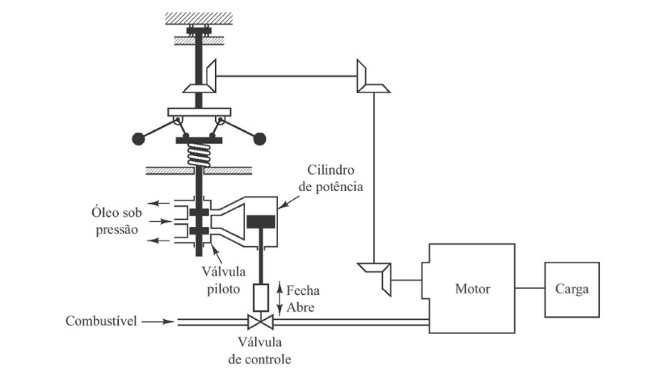
\includegraphics[width=\linewidth]{Figuras/imagem1.JPG} \\
    \end{center}
    \fontsize{10}{12}\selectfont{Fonte: \citeauthor{ogata}, \citeyear{ogata}. }
    
\end{figure}

A Figura~\ref{fig:icone} é uma figura elaborado pelo autor em 2020. Veja como fica a legenda.

\begin{figure}[H] % ht para here, b para     bottom e t para top
    \begin{center}
    \caption{Imagem do autor.} %//não esqueça o ponto final
    \label{fig:icone}
    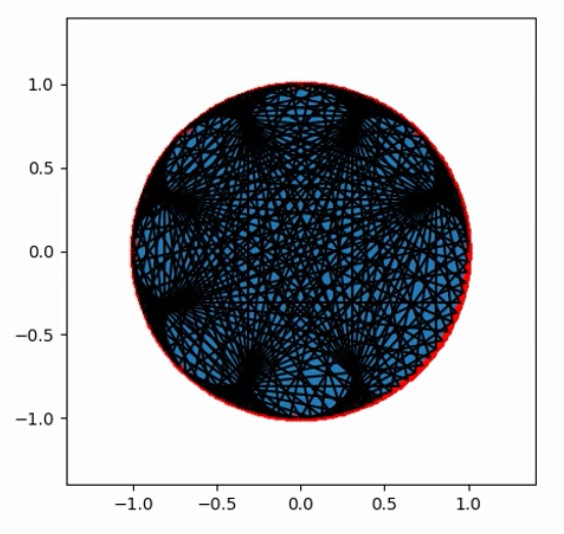
\includegraphics[width=0.5\linewidth]{Figuras/imagem2.jpg} \\
    \end{center}
    \fontsize{10}{12}\selectfont{Fonte: Elaborado pelo autor, \imprimirano. }
    
\end{figure}


A Figura~\ref{fig:ifmg} é uma figura retirada de um site.

\begin{figure}[H] % h! para here, b para bottom e t para top
   \begin{center}
    \caption{Logo do IFMG.} %//não esqueça o ponto final
    \label{fig:ifmg}
    
\includegraphics[width=0.5\linewidth]{Figuras/ifmg.png} \\
    \end{center}
    \fontsize{10}{12}\selectfont{Fonte: \href{https://www.ifmg.edu.br/itabirito}{https://www.ifmg.edu.br/itabirito}. }
\end{figure}

%\par\bigskip % acrescenta um espaço para forçar o texto ser depois da imagem

\dangersign[5ex]  {\color{red}
Obs.: Siga os exemplos deste capítulo sempre que for inserir uma nova figura!
}


O formulário utilizado na pesquisa pode ser encontrado no ANEXO~\ref{anexoA}.

Exemplo de quadro, conforme Quadro~\ref{qd:exemplo}.

\begin{quadro}[htb]
  \centering
  \caption{Exemplo de quadro.}\label{qd:exemplo}
  \begin{tabular}{cp{12cm}}
    \hline \hline &\\[-0.4cm]
    \textbf{Etapas} & \textbf{Descrição} \\
    \hline
    &\\[-0.4cm]
    \textbf{1} & Leitura das regras. \\[0.2cm]
    \textbf{2} & Revisão da literatura de trabalhos correlacionados. \\[0.2cm]
    \textbf{3}& Implementação.\\[0.2cm]
    \textbf{4} & Validação. \\[0.2cm]
    \textbf{5} & Produção científica e/ou documentação.\\[0.2cm]
    \hline \hline
  \end{tabular}
\end{quadro}


Exemplo de cronograma, conforme Tabela~\ref{tb:cronograma}.

\begin{table}[!ht]
     \caption{Cronograma do projeto.}\label{tb:cronograma}
	\centering
	\resizebox{\linewidth}{!}{
		\begin{tabular}{|c|c|c|c|c|c|c|c|c|c|c|c|c|} \hline
		& \multicolumn{12}{c|}{Meses}\\ \cline{2-13}
         \raisebox{1.5ex}{Etapas} & 01 & 02 & 03 & 04 & 05 & 06 & 07 & 08 & 09 & 10 & 11 & 12 \\		\hline
		1&\cellcolor{midgray}&\cellcolor{midgray}&\cellcolor{midgray}&\cellcolor{midgray}&&&&&\cellcolor{midgray}&\cellcolor{midgray}&\cellcolor{midgray}&\\
		\hline
		2&&&\cellcolor{midgray}&\cellcolor{midgray}&\cellcolor{midgray}&&&&&&&\\
		\hline	
		3&&&&\cellcolor{midgray}&\cellcolor{midgray}&\cellcolor{midgray}&&&&&&\\
		\hline			
		4&&&&\cellcolor{midgray}&\cellcolor{midgray}&\cellcolor{midgray}&\cellcolor{midgray}&&&&&\\
		\hline	
		5&&&&&&&&\cellcolor{midgray}&\cellcolor{midgray}&&&\\
		\hline
		
		
		\end{tabular}
		}
\end{table}

\clearpage

\chapter{Resultados} \label{resultado}

Neste capítulo são apresentados os resultados alcançados durante todo o trabalho, bem como uma discussão  e comparação com os resultados encontrados na literatura, destacando a importância desta pesquisa no contexto acadêmico.

A Equação \ref{eq:importante}
apresenta ....
%
\begin{equation}
\label{eq:importante}
    x^2      x^{2x} \cdot y + \vec{a}\times \vec{b} + \int_{a}^{b}x^3 dx = \xi_0 ,
\end{equation}
em que x é uma variável.

Na Equação~\ref{eq:transformada} observa-se que ...
%
\begin{equation}
\label{eq:transformada}
\vec{z} = \begin{bmatrix}
x_d 
\\ 
y_d 
\end{bmatrix} = \begin{bmatrix}
x_c + d\cos\theta
\\ 
y_c + d\sin\theta 
\end{bmatrix},
\end{equation}
em que $d$ é a distância até o centro do objeto.

Outro exemplo de expressão matemática:
%
\begin{equation}
   3\mu_0 \cdot \left \{ \frac{2}{3} \cdot \vec{x}\times \vec{y} \right \} \\
   \int_{x_1}^{x_2}hdx .
\end{equation}

Para as equações seguir também os modelos acima.
%\chapter{Considerações Finais} \label{consideracoes}

%%====== Section ========%
\chapter{Conclusão e Trabalhos Futuros}\label{conclusao}

Nesta sessão são apresentados de forma sucinta os resultados obtidos e um fechamento de todo trabalho desenvolvido.



%%====== Section ========%
\section{Publicações Realizadas}\label{publicacoes}

Caso o trabalho tenha originado publicações é válido acrescentar essa informação no trabalho da seguinte maneira:

Os trabalhos seguintes, que foram originados das metodologias propostas, foram aceitos para apresentação em conferências nacionais:

\begin{enumerate}
   \item Silva, J. Monografia IFMG. 2017, Itabirito - MG
   \item Silva, J. Monografia IFMG. 2016, Itabirito - MG  
\end{enumerate}

%%====== Section ========%
\section{Trabalhos Futuros}\label{trabalhosFuturos}

Apresente propostas para a continuação do seu trabalho....

\vspace{4cm}
\begin{center}
    \Large Bom trabalho! 
    
    \dSmiley[5][yellow]
\end{center}



% ----------------------------------------------------------
% -- Elementos Pós-Textuais: -------------------------------
\postextual  
\bibliography{bibliografia} % Referências bibliográficas
%-------------------------------------------------------------
%---------------------- Apêndices ----------------------------
%-------------------------------------------------------------

\begin{apendicesenv}
%\partapendices  % Indica o início dos Apendices
\chapter{Informações para complementar o texto}
\lipsum[8]


\chapter{Como apresentar os dados de pesquisa}

\lipsum[8]

\end{apendicesenv}
%----------------------------------------------------------------
%---------------------- Anexos ----------------------------------
%----------------------------------------------------------------

\begin{anexosenv}
%\partanexos   % indica o início dos anexos
\chapter{Mapa de unidades do IFMG.}
\label{anexoA}

Note que os  Anexos são  \textbf{documentos  que não foram  elaborados  pelo  autor},  que  servem  também  de  fundamentação, comprovação ou ilustração do trabalho, como leis, mapas, ilustrações etc .

\begin{figure}[H] % h! para here, b para bottom e t para top
   \begin{center}
    \caption{Mapa de unidades do IFMG.} %//não esqueça o ponto final
    \label{fig:mapas}
    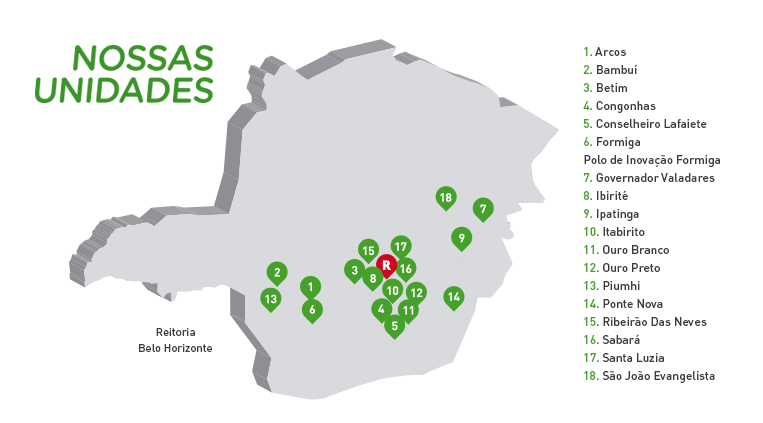
\includegraphics[width=1\linewidth]{Figuras/mapasitenovonov2018b.png} \\
    \end{center}
    \fontsize{10}{12}\selectfont{Fonte: \href{https://www.ifmg.edu.br/portal/sobre-o-ifmg/mapasitenovonov2018b.png}{https://www.ifmg.edu.br/portal/sobre-o-ifmg}. }
\end{figure}



\end{anexosenv}

%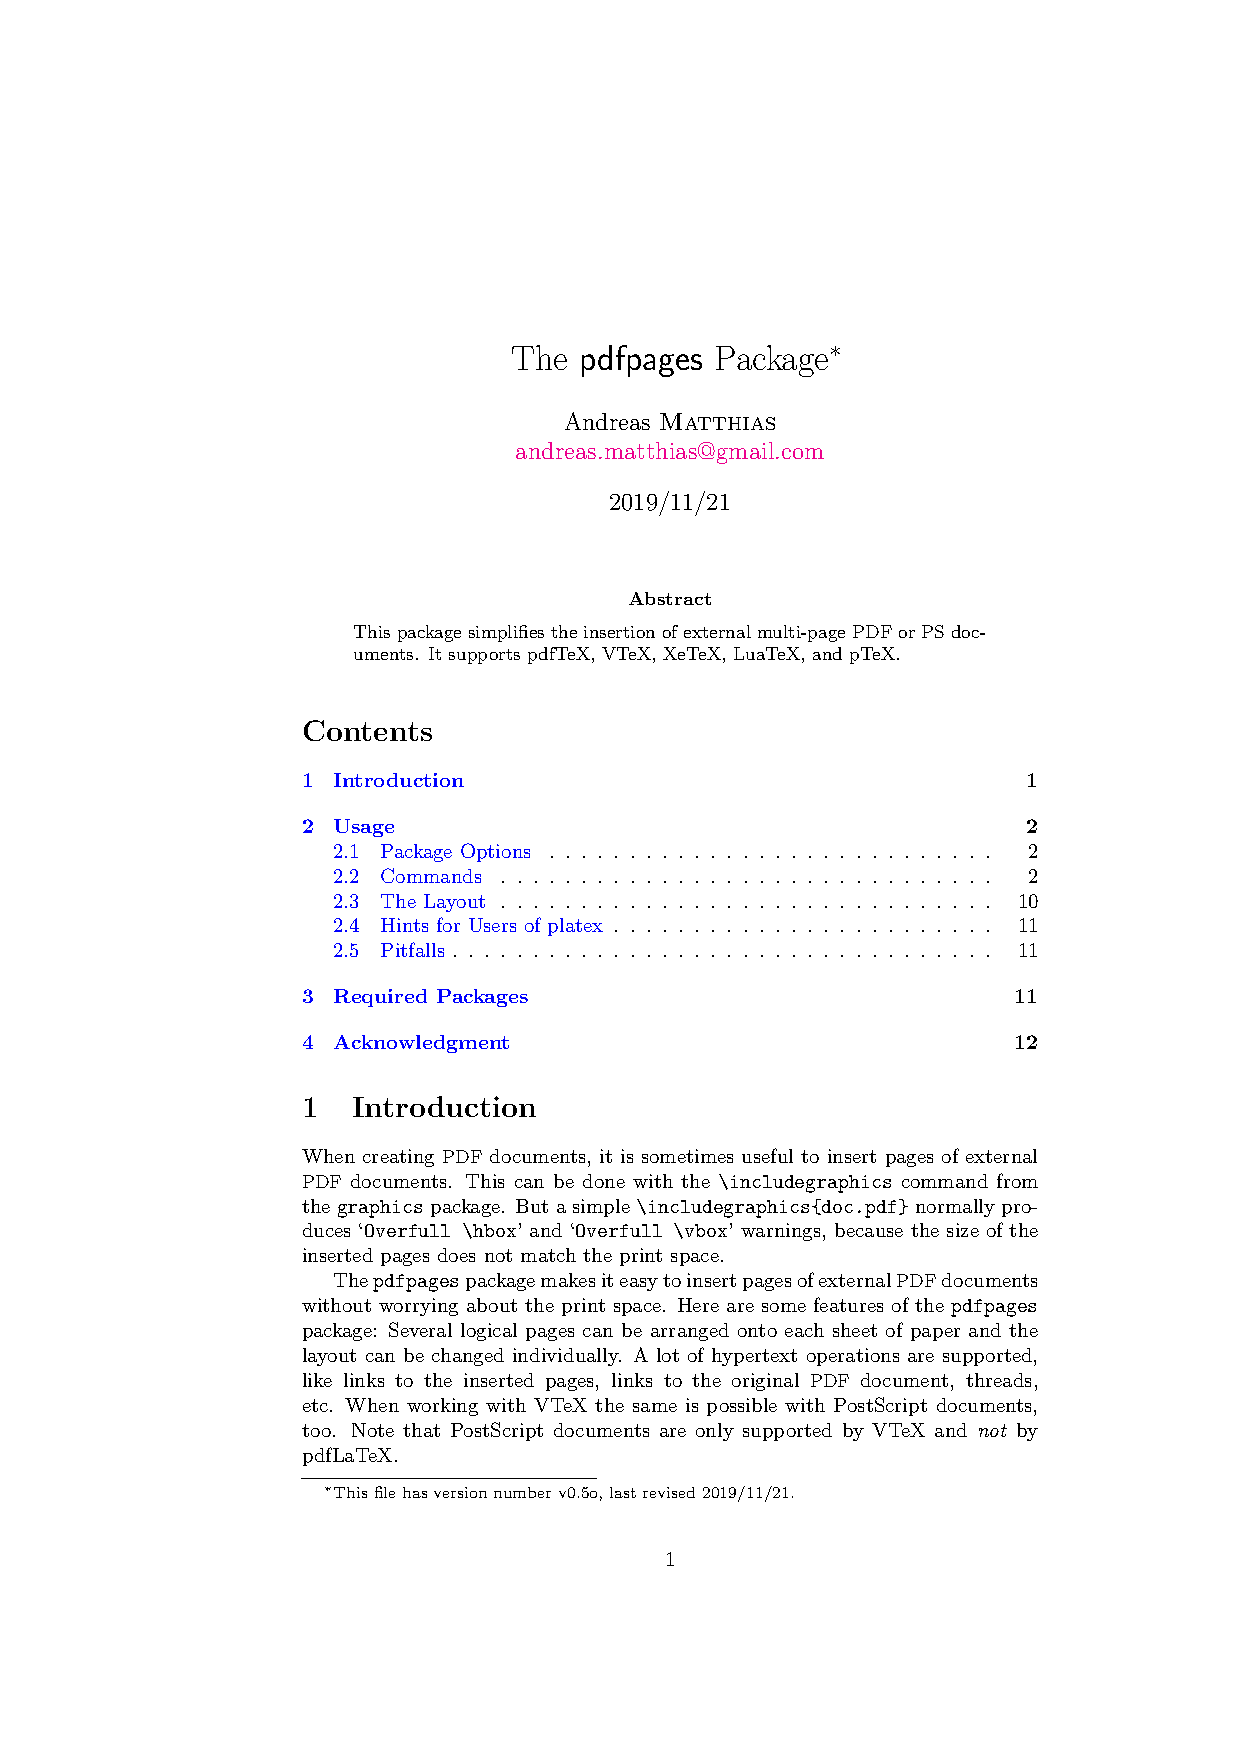
\includepdf[pages={1,3-5}]{PosTextuais/includepdfpages.pdf}
%\phantompart  \printindex  % Indice Remissivo
% ----------------------------------------------------------
\end{document}  % fim do documento
